\documentclass[11pt, oneside]{article} 
\usepackage{geometry}
\geometry{letterpaper} 
\usepackage{graphicx}
	
\usepackage{amssymb}
\usepackage{amsmath}
\usepackage{parskip}
\usepackage{color}
\usepackage{hyperref}

\graphicspath{{/Users/telliott/Github/calculus_book/png/}}
% \begin{center} 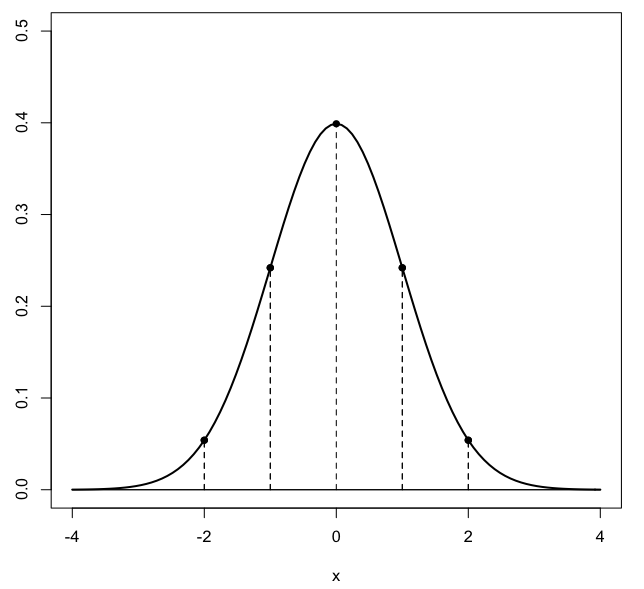
\includegraphics [scale=0.4] {gauss3.png} \end{center}

\title{Slope of a parabola}
\date{}

\begin{document}
\maketitle
\Large

This chapter is an extended example in three parts as a further taste of analytic geometry.  We show how to find the slope of parabola at any point using classical methods.

\subsection*{part 1}
Consider the simplest parabola:  $y = x^2$.

The point $(1,1)$ is on the curve, because $(x = 1, y = 1)$ satisfies the equation $y = x^2$.

\begin{center} 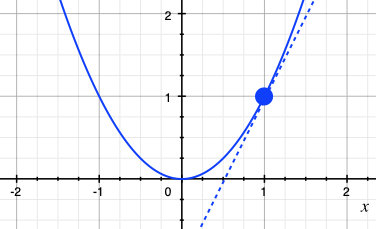
\includegraphics [scale=0.50] {para11.png} \end{center}

Suppose we know that the slope of the tangent to the curve at the point $(1,1)$ is equal to $2$.

(Using calculus to find this result is trivial, we'll also show a non-calculus method in part three, below).  

The equation of the tangent line is
\[ y' - y = m(x' - x) \]
Plugging in for $(x,y) = (1,1)$:
\[ y' - 1 = 2(x' - 1) \]
\[ y' = 2x' - 1 \]
which we can write for generalized $x$ and $y$ as
\[ y = 2x - 1 \]

Now suppose that we knew only the parabola and this slope, but we did not know the point where the tangent meets the curve, and so do not know the $y$-intercept.

We have the equation of a line:
\[ y = 2x + b \]
We are going to use the symbol $b$ a lot in this chapter, for the quadratic equation.  There is nothing about vertices or centers off the origin, so let us substitute $k$ as the $y$-intercept:
\[ y = 2x + k \]

We seek points which are simultaneously on the line and the curve.  They must satisfy both equations.

So, substitute for $y$ from the equation for the curve:
\[ x^2 = 2x + k \]
\[ x^2 - 2x - k = 0 \]

Now look at the quadratic formula we would use to solve this equation for $x$:
\[ x = \frac{-b \pm \sqrt{b^2 - 4ac}}{2a} \]

Since this is a tangent line, we seek the values for which this expression has only a single solution.  The tangent "kisses" the curve at a single point.

That happens when the part under the square root (called the discriminant) is equal to zero.

\[ b^2 - 4ac = 0 \]
\[ b^2 = 4ac \]
\[ (-2)^2 = 4(-k) \]
\[ k = -1 \]
Therefore, the equation of the tangent line is $y = 2x - 1$, which matches what we had before.

In general, $y = 2x + k$ is a \emph{family} of lines.  For $k = -1$, there is a single solution for $x$ to be both on the line and the parabola.  For $k < -1$, there are no solutions, while for $k > -1$ there are two solutions, because the line actually traces out a secant of the parabola, passing through the curve at two points.

\subsection*{part 2}
Now suppose we have the same parabola and a point not on the parabola, but in the plane and outside of the "cup" of the parabola, such as $(3,5)$.  We seek the equations of tangent lines to the parabola that go through this point.  
\begin{center} 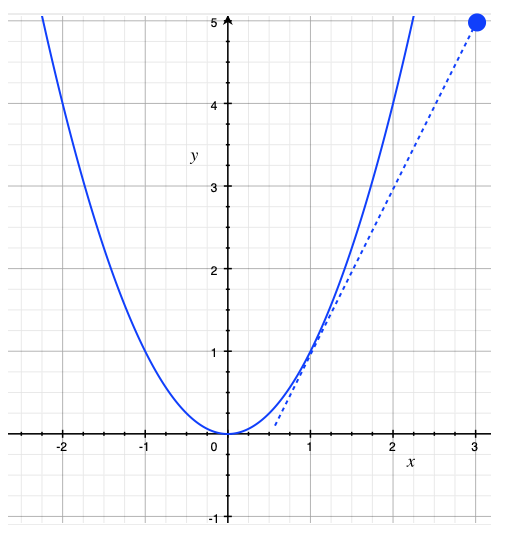
\includegraphics [scale=0.50] {para12.png} \end{center}

There will be two of them.  We show just one.

The equations of lines passing through this point, with different slopes $m$ are given by:

\[ y - y' = m(x - x') \]
\[ y - 5 = m(x - 3) \]

Since values of $(x,y)$ are both on the line and the parabola $y=x^2$:
\[ x^2 - 5 = mx - 3m \]
\[ x^2 - mx + (3m - 5) = 0 \]

Solutions are given by the quadratic equation.  The value of the slope $m$ giving a single solution (zero discriminant) is:
\[ (-m)^2 - 4(3m - 5) = 0 \]
\[ m^2 - 12m + 20 = 0 \]
\[ (m - 2)(m - 10) = 0 \]
\[ m = 2, \ \ \ m = 10 \]

We knew the first one already, because the point $(3,5)$ is on the line $y = 2x - 1$.  This is the tangent to the curve at $(1,1)$, which has slope $m = 2$.
\begin{center} 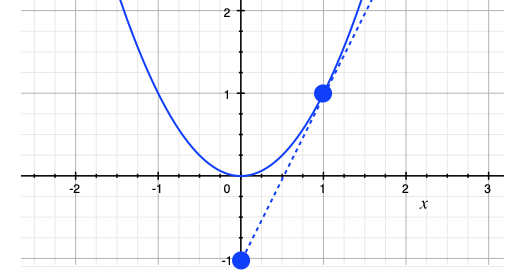
\includegraphics [scale=0.50] {para13.png} \end{center}

Actually, there is always another solution.  Any vertical line (with infinite slope) passes through only a single point on the parabola.

Basically what this amounts to is that in the equation
\[ x = \frac{m \pm \sqrt{(-m)^2 - 4(3m - 5)}}{2} \]

as $m$ gets very large, only the term $(-m)^2$ matters under the square root, so we have
\[ x = \frac{m \pm \sqrt{(-m)^2}}{2} \]
and as $m \rightarrow \infty$, $m - \sqrt{m^2} \rightarrow 0$.

\subsection*{part 3}
Now suppose we have again the same parabola and a point on it such as $(x,y)$.  

To find the equation of a tangent line through that point we need the slope $m$:
\[ y - y' = m(x - x') \]

To find points that satisfy both equations, plug in from $y = x^2$:
\[ x^2 - y' = m(x - x') \]
\[ x^2 - mx + (mx' - y') = 0 \]
Solve for $x$ using the quadratic equation.  

\[ x = \frac{m \pm \sqrt{m^2 - 4(mx' - y')}}{2} \]

We seek a slope where there is only a single $x$ that satisfies the equation.  Again the discriminant should be zero.
\[ m^2 = 4(mx' - y') \]
\[ m^2 - 4mx' + 4y' = 0 \]

To find the slope, solve for $m$.  Again, using the quadratic, but we don't need to write the whole thing.  There is a unique tangent line, thus a unique slope.  Therefore, the discriminant should again be equal to zero.

That leaves, simply, the part of the quadratic formula that is \emph{not} under the square root:
\[ - \frac{b}{2a} = \frac{4x'}{2} = 2 x' \]

The slope of the tangent line is $2x'$ and in particular, at the point $(1,1)$, the slope is equal to $2$.

\subsection*{important note}

If you work through this problem for a parabola with shape factor $a$, you will find that the equation for the slope is $m = 2ax$.

\subsection*{alternate solution}
\begin{center} 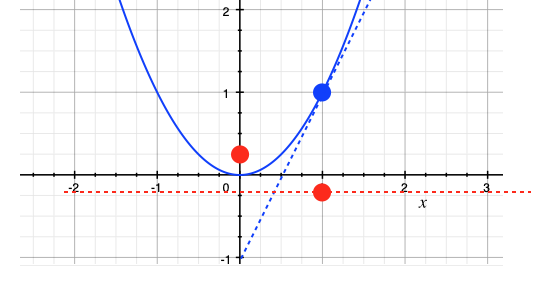
\includegraphics [scale=0.50] {para14.png} \end{center}

A parabola is defined geometrically by its focus, which is the point $(p,0)$ for a centered parabola.

The focus is paired with a directrix, which is the line $y = -p$ for a vertex at the origin.  

All points on the parabola lie at the same distance $d$ from the focus and the directrix.

A relatively advanced fact about the parabola is that any tangent line intersects the $y$-axis at the same distance $d$ from the focus.

\begin{center} 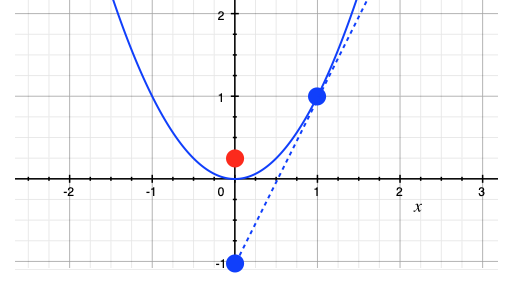
\includegraphics [scale=0.50] {para15.png} \end{center}

Which is to say that if we draw a triangle in the above diagram using the two blue points and one red one, the two blue points are the vertices of equal angles and the triangle formed is isosceles.

For $y = x^2$, consider the point $(x,x^2)$, and find the distance to the focus squared as 
\[ d^2 = (x)^2 + (x^2 - p)^2 \]
\[ d^2 = x^2 + x^4 - 2x^2p + p^2 \]

Call the $y$-intercept $k$ so then 
\[ k + d = p \]
\[ d^2 = p^2 - 2pk + k^2 \]

Equating the two expressions:
\[ p^2 - 2pk + k^2 = x^2 + x^4 - 2x^2p + p^2 \]
\[ k^2 - 2pk = x^2(1 + x^2 - 2p)  \]

In this case, we know $x = 1$ and $p = 1/4$ so
\[ k^2 - \frac{k}{2} - (2 - \frac{1}{2}) = 0 \]

We factor to obtain:
\[ (k + 1)(k - \frac{3}{2}) = 0 \]

$k = -1$ was our solution above.

[ ?? What is the significance of the other solution?? ]

\end{document}